\subsection{由赋值定义的拓扑}

设 K 是一个未必交换的域，v 是 K 上的一个赋值，G 是全序群 \(v(\mathbf{K}^{*})\) 。对一切 \(\alpha \in G\) ，设 \(V_{\alpha}\) 是由这样的 \(x \in K\) 组成的集合：\(v(x) > \alpha\) ；这个集合是 K 的加法子群（ \(\S 3\) 第 1 节）。K 上存在唯一的拓扑 \(T_{v}\) ，使诸 \(V_{\alpha}\) 构成 0 的基本邻域系（《一般拓扑学》第三章 \(\S 1\) 第 2 节例）。v 为非真的，当且仅当 \(T_{v}\) 是离散拓扑。

引理 1. 设 \(x \in \mathbf{K}^*\) ，\(y \in \mathbf{K}^*\) ，\(\alpha \in \mathbf{G}\) 。若

\[
v (x - y) > \sup (\alpha + 2 v (y), v (y)),
\]

则 \(v(x^{-1} - y^{-1}) > \alpha\) 。

\(x^{-1} - y^{-1} = x^{-1}(y - x)y^{-1}\) ，因而

\[
v (x ^ {- 1} - y ^ {- 1}) = v (x - y) - v (x) - v (y).
\]

若 \(v(x - y) > v(y)\) ，则 §3 第 1 节命题 1 蕴含 \(v(x) = v(y)\) ，因为 \(x = y + (x - y)\) 。此外，若 \(v(x - y) > \alpha + 2v(y)\) ，则

\[
v (x ^ {- 1} - y ^ {- 1}) > \alpha + 2 v (y) - 2 v (y) = \alpha .
\]

命题 1. 拓扑 \(\mathcal{T}_{v}\) 是 Hausdorff 的，且与 K 上的域结构相容。若给 G 以离散拓扑，则映射 \(v: \mathbf{K}^{*} \to \mathbf{G}\) 是连续的。

设 \(x \in \mathbf{K}^*\) ，\(\alpha = v(x)\) ；则 \(x \notin \mathrm{V}_{\alpha}\) ，这表明 \(\mathcal{T}_v\) 是 Hausdorff 的。对一切 \(x_0 \in \mathbf{K}\) 与 \(\alpha \in \mathbf{G}\) ，存在 \(\beta \in \mathbf{G}\) 使得 \(x_0\mathrm{V}_{\beta} \subset \mathrm{V}_{\alpha}\) 且 \(\mathrm{V}_{\beta}x_0 \subset \mathrm{V}_{\alpha}\) （取 \(\beta \geqslant \alpha - v(x_0)\) 即可）。另一方面，若 \(\alpha \geqslant 0\) ，则 \(\mathrm{V}_{\alpha}\mathrm{V}_{\alpha} \subset \mathrm{V}_{\alpha}\) 。《一般拓扑学》第三章 § 6 第 3 节的公理 \((\mathrm{AV}_{\mathrm{I}})\) 与 \((\mathrm{AV}_{\mathrm{II}})\) 既已满足，\(\mathcal{T}_{v}\) 便与 K 上的环结构相容。设 \(x_{0} \in \mathrm{K}^{*}\) ；若 \(x \in \mathrm{K}^{*}\) 满足 \(v(x - x_{0}) > \sup (\alpha + 2v(x_{0}), v(x_{0}))\) ，则 \(v(x^{-1} - x_{0}^{-1}) > \alpha\) （引理 1），这表明 \(x \mapsto x^{-1}\) 是连续的，因而 \(\mathcal{T}_{v}\) 与 K 上的域结构相容。最后，仅条件 \(v(x - x_{0}) > v(x_{0})\) 就蕴含 \(v(x) = v(x_{0})\) （§ 3 第 1 节命题 1），因此若给 G 以离散拓扑，则映射 \(v: \mathrm{K}^{*} \to \mathrm{G}\) 是连续的。

设 \(\alpha \in G\) ，\(V_{\alpha}^{\prime}\) 是由这样的 \(x \in K\) 组成的集合：\(v(x) \geqslant \alpha\) 。若 \(\beta < \alpha\) ，则 \(V_{\beta} \supset V_{\alpha}^{\prime} \supset V_{\alpha}\) 。若 \(v\) 不是非真的，则由此可知诸 \(V_{\alpha}^{\prime}\) 构成 \(\mathcal{T}_{v}\) 下 0 的基本邻域系。

诸 \(V_{\alpha}\) 与诸 \(V_{\alpha}^{\prime}\) 是开的加法子群，因此在 K 中是闭的，因而拓扑域 K 是全不连通的。由于 v 的环的每个非零理想都包含某个 \(V_{\alpha}\) ，它在 K 中既开又闭。因此 v 的剩余域上的商拓扑是离散的。

\pandocbounded{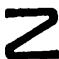
\includegraphics[keepaspectratio]{images/part003_6b42bd98.jpg}}

设 A 是 v 的环。若 v 是离散的，则 §3 第 6 节命题 8 表明 \(T_{v}\) 在 A 上诱导的拓扑是 m(A)-进拓扑。一般情形并非如此（习题 4）。

命题 2. 设 K 是一个未必交换的域，v 是 K 上一个非真的赋值，A 是 v 的环，m 是 v 的理想。赋以拓扑 \(\mathcal{T}_v\) 的 K 为局部紧的，当且仅当下列条件成立：

\begin{enumerate}
\def\labelenumi{(\roman{enumi})}
\item
  K 是完备的；
\item
  v 是离散的；
\item
  剩余域 \(\kappa(A)\) 是有限的。
\end{enumerate}

若是这样，则 A 是紧的。

设 K 是局部紧的。那么它是完备的（《一般拓扑学》第三章 § 3 第 3 节命题 4 的推论 1）；此外存在 0 的一个紧邻域，它包含某个邻域 \(\mathbf{V}_{\alpha}^{\prime}\) ，其中 \(\alpha\) 属于 \(v\) 的值群；换言之，存在 \(a \neq 0\) 在 \(\mathbf{K}^*\) 中，使得 A.a 是紧的，于是 \(\mathrm{A} = (\mathrm{A}.a)a^{-1}\) 是紧的。由于 A 的每个理想 \(\mathfrak{b} \neq (0)\) 都是开的，A/b 是紧的且离散的（《一般拓扑学》第三章 § 2 第 5 节命题 14），因而是有限的，特别地 \(\kappa(\mathrm{A}) = \mathrm{A}/\mathfrak{m}\) 是有限的。此外，对 \(y \neq 0\) （在 \(\mathfrak{m}\) 中），环 A/Ay 是有限的，故 A 中含 Ay 的理想只有有限多个，从而形如 \(v(x)\) 且满足

\[
0 <   v (x) \leqslant v (y)
\]

的元素组成的集合 P 是有限的；由于 \(v(\mathbf{K}^{*})\) 是全序的，P 有最小元素 \(\gamma\) 。于是对一切 \(x \in A\) （满足 \(v(x) > 0\) ），或者 \(v(x) > v(y) \geqslant \gamma\) ，或者 \(v(x) \leqslant v(y)\) 而按定义有 \(v(x) \geqslant \gamma\) ，所以 \(\gamma\) 是 \(v(\mathbf{K}^{*})\) 中 >0 的元素中最小的。由于 P 有限，存在最大整数 \(m \geqslant 0\) 使得 \(m_{\gamma} \in P\) ，于是 \(m\gamma \leqslant v(y) < (m + 1)\gamma.\) 由此得出 \(0 \leqslant v(y) - m\gamma < \gamma\) ，由 \(\gamma\) 的定义这蕴含 \(v(y) = m\gamma.\) 因此 \(v(\mathbf{K}^{*}) = \mathbf{Z}. \gamma\) ，赋值 \(v\) 是离散的。

反之，设条件 (i)、(ii)、(iii) 成立。可以只限于 v 是赋范的情形；设 u 是 v 的一个单值化元。那么 \(\kappa(\mathbf{A}) = \mathbf{A}/\mathbf{A}u\) ，因而 A/Au 是有限的。由于 \(x \mapsto xu^{n}\) 通过取商定义了加法群 A/Au 到 \(Au^{n}/Au^{n+1}\) 上的一个同构，故 \(A/Au^{j}\) 对一切 \(j \geqslant 0\) 是有限的。由于 A 在 K 中是闭的，它是完备的，因而同构于诸 \(A/Au^{j}\) 的逆极限（《一般拓扑学》第三章 §7 第 3 节命题 2），因此是紧的。既然 A 在 K 中是开的，由此可知 K 是局部紧的。

注. 注意在此证明中只需假设 A 是完备的。

我们将在 § 9 中看到，满足命题 2 中条件的域 K 有一个中心，它或者是 p-进域的有限代数扩张，或者是有限域上的形式幂级数域 \(\mathbf{F}_{q}((\mathbf{T}))\) ；此外 K 在其中心上是有限秩的。

